\chapter{Numerical modelling of granular flows}

\ifpdf
    \graphicspath{{Chapter3/figs/raster/}{Chapter3/figs/pdf/}{Chapter3/figs/}}
\else
    \graphicspath{{Chapter3/figs/vector/}{Chapter3/figs/}}
\fi

\section{Introduction}

The dynamics of a homogeneous granular flow involve at least three distinct 
scales: the \textit{microscopic scale}, which 
is characterised by the contact between grains, the \textit{meso-scale} that 
represents micro-structural effects such as grain rearrangement, and the 
\textit{macroscopic scale}, where geometric correlations can be observed (see 
Figure~\ref{fig:multiscale}). Conventionally, granular flows are modelled as a 
continuum because they exhibit many collective phenomena. However, on a grain 
scale, the granular materials exhibit complex solid-like and/or fluid-like 
behaviour. Recent studies, however, suggest that a continuum law may be unable 
to capture the effect of inhomogeneities at the grain scale level, such as 
orientation of force chains, which are micro-structural effects. Discrete 
element methods (DEM) are capable of simulating these micro-structural effects, 
however they are computationally expensive. In the present study, a multi-scale 
approach is adopted, using both DEM and continuum techniques, to better 
understand the rheology of granular flows and the limitations of continuum 
models.

\begin{figure}[tbhp]
\centering
\includegraphics[width=0.95\textwidth]{multiscale}
\caption{Multi-scale modelling of granular materials}
\label{fig:multiscale}
\end{figure}

\subsection{Voronoi Tesselation}
\begin{figure}[tbhp]
\centering
\begin{subfigure}[b]{0.95\textwidth}
\centering
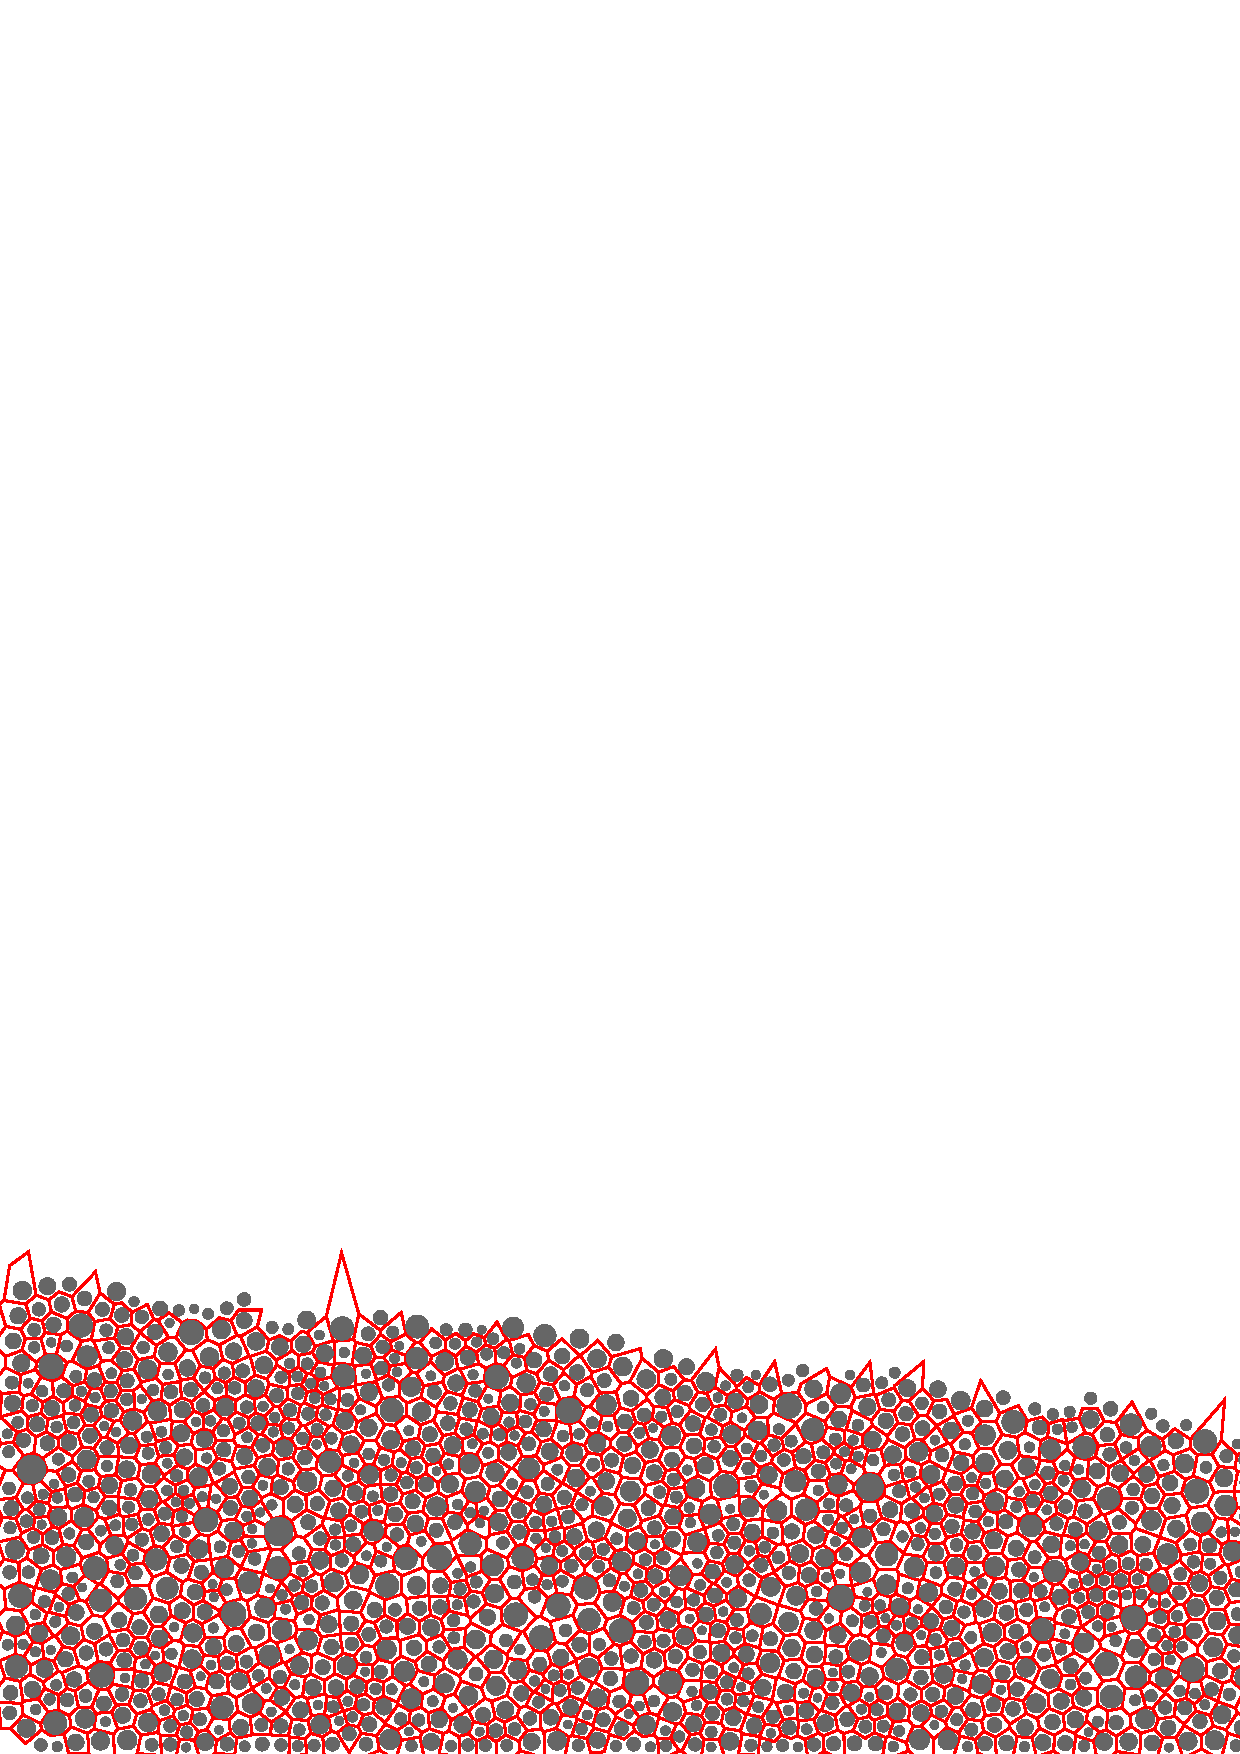
\includegraphics[width=\textwidth]{tesselation}
\caption{Voronoi Tesselation}
\label{fig:tesselation}
\end{subfigure}
\\
\begin{subfigure}[b]{0.95\textwidth}
\centering
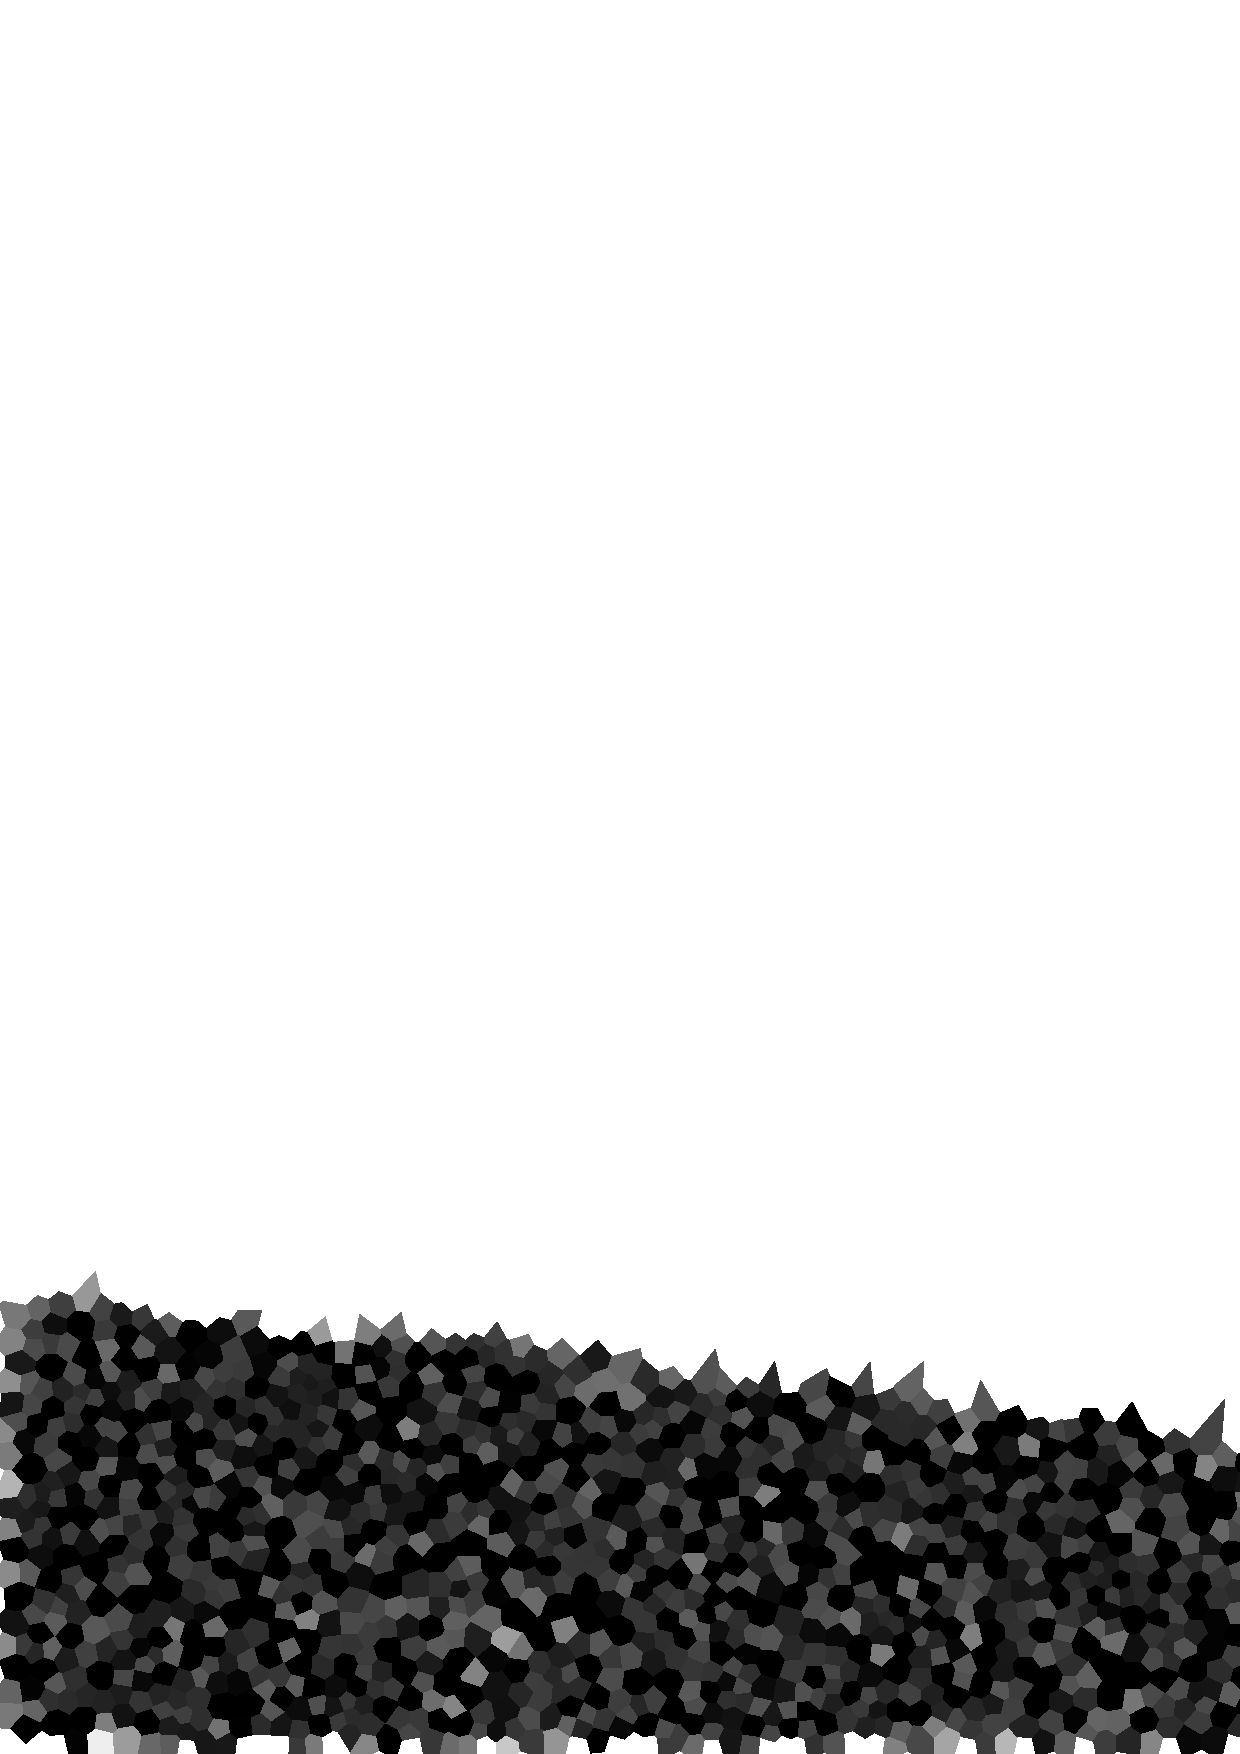
\includegraphics[width=\textwidth]{local_density}
\caption{Local packing density (dark - dense and light - loose)}
\label{fig:local_density}
\end{subfigure}
\caption{Voronoi tessellation to average bulk properties}
\label{fig:voro}
\end{figure}
